\section{Introduction}

Product categorization \cite{ding2002goldenbullet} is a specialized 
text classification task that classifies product titles or descriptions 
into a pre-defined taxonomy of categories.
As businesses expand, major e-commerce platforms (\textit{e.g.,} Amazon and Alibaba) are encountering increasingly complex scenarios, 
% more complicated scenario. 
% bigger challenge 
where there are multiple domain-specific category taxonomies and each of them evolves dynamically over time.
We define it as \textit{$\mathbf{D}$ynamic $\mathbf{M}$ulti-Domain $\mathbf{P}$roduct $\mathbf{C}$ategorization} ($\mathbf{DMPC}$), which simultaneously considers the following \textbf{multi-domain taxonomies} and \textbf{taxonomy evolving} challenges.

In real-world businesses, e-commerce platforms usually maintain \textbf{multiple} business lines with relatively independent \textbf{taxonomies}.
These business lines are catering for different customer demands or
specific domain applications, 
for example, one provides express delivery while another specializes in 
low-price bargains.
Multiple business domains correspond to different category taxonomy structures, with various depths and distinct literal expressions of category names. 
Conventional industry approaches train separate classifiers on each domain, which under-utilize the cross-domain data and their shared knowledge while 
raising the expenses of maintenance.
Meanwhile, with the expansion and reorganization of businesses, 
each category \textbf{taxonomy} keeps \textbf{evolving} as well, where 
old categories might be deleted or integrated and new categories are possibly added.
Conventional multi-class classifiers need to be re-trained every time 
taxonomy changes, which 
% is 
% less robust 
% vulnerable
% towards taxonomy evolving issues.
disrupts the operation and further diminishes the maintenance efficiency.
% While training and maintaining separate models for each business line is laborious, 
% rich resources 
% common rules
% in cross-domain data and their shared knowledge 
% are hardly exploited as well.

% To jointly circumvent the above issues, 
To mitigate \textbf{taxonomy evolving} issues, 
intuitively, we reformulate the canonical text classification problem as a text relevance matching problem. Moreover, to ensure both accuracy and online efficiency, we propose a two-stage \textit{Taxonomy-agnostic Label Retrieval} ($\mathsf{TaLR}$) framework (see \figref{fig:pipeline}) capturing semantic similarity between a product title and its corresponding category names in the vector space, where candidate categories are first retrieved and then reranked for the final prediction.
This reformulation is especially beneficial for evolving and newly added (zero-shot) categories as textual semantics are incorporated. 

% For example, despite the integration of [$\mathtt{Sardine}$] and [$\mathtt{Silver}\,\mathtt{Sillago}$] into [$\mathtt{Sillago}$], their textual meanings are barely drifted.
% , and the meaning of incoming class labels like [$\mathtt{Fish Roe}$] and [$\mathtt{Sashimi}$] could be captured in textual semantics as well. 

% However, pure textual matching approaches are insufficient for accurate categorization when some hidden concept knowledge is ignored.
% For example, \textit{Haagen-Dazs Red Wine Flavor} might be wrongly categorized into [$\mathtt{Red\,Wine}$] instead of the correct [$\mathtt{Ice\,Cream}$], mainly because the keyword \textit{Red Wine} in the lexical surface form 
% \textbf{dominates other information} in the semantic matching score and thus 
% leads the model to a skewed direction. Here, \textit{Haagen-Dazs} is one of the fine-grained concepts which are easily ignored by pure semantic matching.
% in general semantic space.
To leverage cross-domain data in \textbf{multi-domain taxonomies} challenge, we devise two plug-in modules 
in both stages 
to enhance $\mathsf{TaLR}$'s domain transferability. These modules are centralized with ``meta concepts'' that appear in 
the product titles, which represent fine-grained keyword knowledge 
shared across domains (Appendix~\ref{sec:datasetdetails}).
% We observe that there are fine-grained keywords in product titles which are usually in short span and exist cross-domain. 
% We term them as meta concepts, as depicted in \figref{fig:pipeline}, which resemble the shared keyword knowledge across domains.
% We assume that leveraging cross-domain knowledge with the help of meta concepts can boost \textbf{knowledge integration} (\S\ref{sec:all res}), and therefore we consider integrating the extracted concept knowledge in both stages of $\mathsf{TaLR}$ framework. 
% Since our concepts are constructed over all domains, the knowledge from \textbf{multi-domain taxonomies} can be jointly leveraged when we jointly training. 
% The concept knowledge is utilized in both stages of $\mathsf{TaLR}$. 
\begin{figure*}[th] \centering
    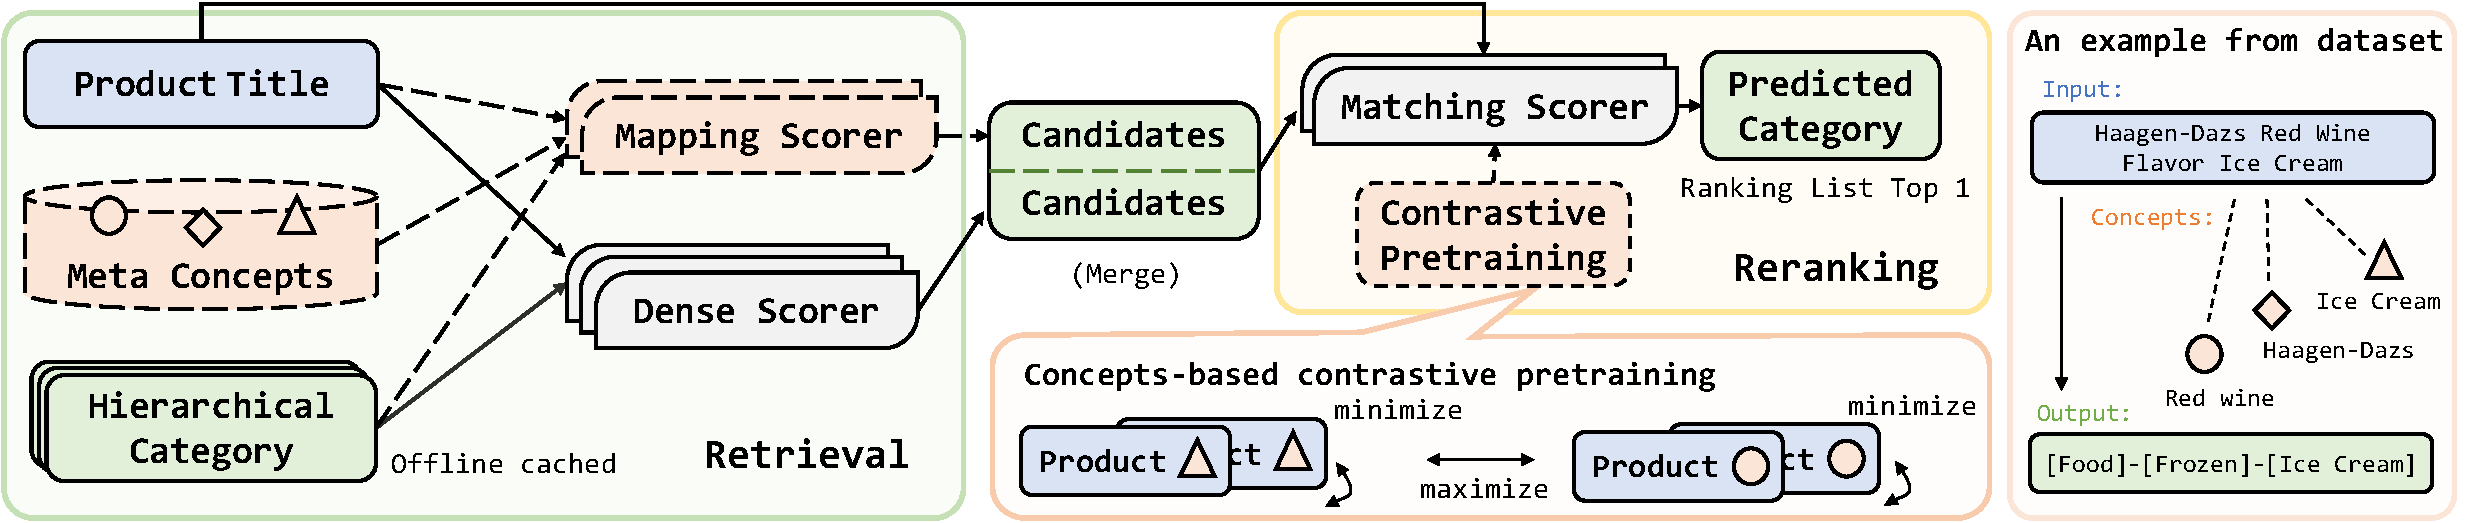
\includegraphics[width=\textwidth]{pipeline}
    \caption{An overview of $\mathsf{TaLR}$ framework, containing \textit{Retrieval} and \textit{Reranking} stages. We show an example from our released dataset, in which the input is a product title with its meta concepts, and the output is its corresponding hierarchical category. In \textit{Retrieval} stage, two lists of category candidates are sampled from mapping scorer and dense scorer. In the \textit{Reranking} stage, merged category candidates are ranked by a matching scorer with contrastive information. Dark dashes refer to plug-in modules. }
    % \KZ{The sample from the dataset
% in the figure is not discussed in the main text. What dataset are you talking about? And it might confuse with ``we sample two groups of candidates...'' in the caption.}
    % \xiujie{it seems a little bit weird to put ``A sample from dataset'' in the center of the figure. may be split this figure into (a) (b)?. for the contrastive learning part, maybe add a ``minimize''?}
    \label{fig:pipeline}
\end{figure*}
As is shown in \figref{fig:pipeline}, in the \textit{retrieval} stage, besides the dense 
retrieval based on 
vector similarity (dense scorer), the statistical co-occurrence probability between meta concepts and 
category labels are exploited as well (mapping scorer) . 
% we design a heuristic strategy to ensemble the vector matching candidates. 
In the \textit{reranking} stage, meta concepts are incorporated with 
category labels as supervision signals for the contrastive pretraining 
of the scoring model (matching scorer). 
While the mapping scorer complements the superficial semantic dense retrieval with cross-domain commonsense knowledge, contrastive pretraining directly optimizes the vector space improving inter-domain alignment and uniformity. Details are given in \secref{sec:mapping} and \secref{sec:contrastive}.
% \TODO{introduce intuition instead of methods, introduce dataset}

In summary, our contributions are:
(1) For the first time, we address the $\mathbf{DMPC}$ problem and release 
the corresponding multi-domain datasets in Chinese. 
(2) We propose a unified $\mathsf{TaLR}$ framework equipped with two well-designed plug-in modules empowered with meta concepts, which is robust and efficient 
against the two challenges in $\mathbf{DMPC}$ problem.
% the effectiveness of them is validated in \S\ref{sec:all res}. 
(3) Offline experiments on our annotated real-world $\mathbf{DMPC}$ datasets show 
$\mathsf{TaLR}$'s ability to effectively transfer knowledge across domains 
and generalize to new domains. The unified $\mathsf{TaLR}$ outperforms three 
separately-trained SOTA classifiers by 1.65\% on overall accuracy and 
maintains satisfactory accuracy in taxonomy evolving conditions.
% , and $\mathsf{TaLR}$ speed 10$\times$ up against its counterpart when the number of classes grows. 
Online experiments reaffirm its efficacy with a 5\% increase in seasonal purchase revenue.
